% ARPEGOS:  Automatized Roleplaying-game Profile Extensible Generator Ontology based System %
% Author : Alejandro Muñoz Del Álamo %
% Copyright 2019 %

% Chapter 3: Planificación del Proyecto %

\chapter{Antecedentes}
\thispagestyle{chapterpage}

Los antecedentes del proyecto son una síntesis conceptual de las 
investigaciones realizadas previamente sobre el problema que se 
desea abordar, así como la propuesta realizada para solventar dicho 
problema, y las metodologías analizadas para el desarrollo. 

% Import Section%
% ARPEGOS:  Automatized Roleplaying-game Profile Extensible Generator Ontology based System %
% Author : Alejandro Muñoz Del Álamo %
% Copyright 2019 %

% Section 2.2: Estado del Arte %

\section{Estado del Arte} \label{Estado_Arte}
Con el objetivo de simplificar el proceso de creación de personajes en los juegos de rol tradicionales, se han originado 
multitud de aplicaciones con diferentes funciones y finalidades. Algunas de las aplicaciones son referencias completas de 
los juegos, que sirven como elementos de consulta accesibles, rápidos y precisos. Un ejemplo de ello es 
\textit{\textbf{5e Character}}, mostrada en las figuras \ref*{5e_Character1} y \ref*{5e_Character2} que es una referencia 
completa de personajes para \textit{Dragones y Mazmorras, 5ª Edición}.\medskip

Estas aplicaciones ofrecen información del juego de manera accesible, pero no permiten aprovechar la 
digitalización de ésta para otros usos. Permiten realizar búsquedas rápidas, pero tampoco suelen disponer de 
toda la información del juego, de manera que para poder hacer consultas del juego completo es necesario 
acceder al libro del juego o hacer uso de más aplicaciones. Además, son aplicaciones que sólo pueden 
ser útiles para una versión específica del juego, ya que las versiones nuevas de los juegos de rol suelen 
incluir una gran cantidad de cambios. Aún así, éstas pueden no resultar obsoletas al momento de surgir la 
nueva versión, pues suele haber un período de transición entre versiones bastante amplio.
\newpage
% https://play.google.com/store/apps/details?id=com.dungeon.dev.a5echaracter&hl=en_US

\begin{figure}[H]
    \centering
    \begin{minipage}{0.38\textwidth}
        \centering
        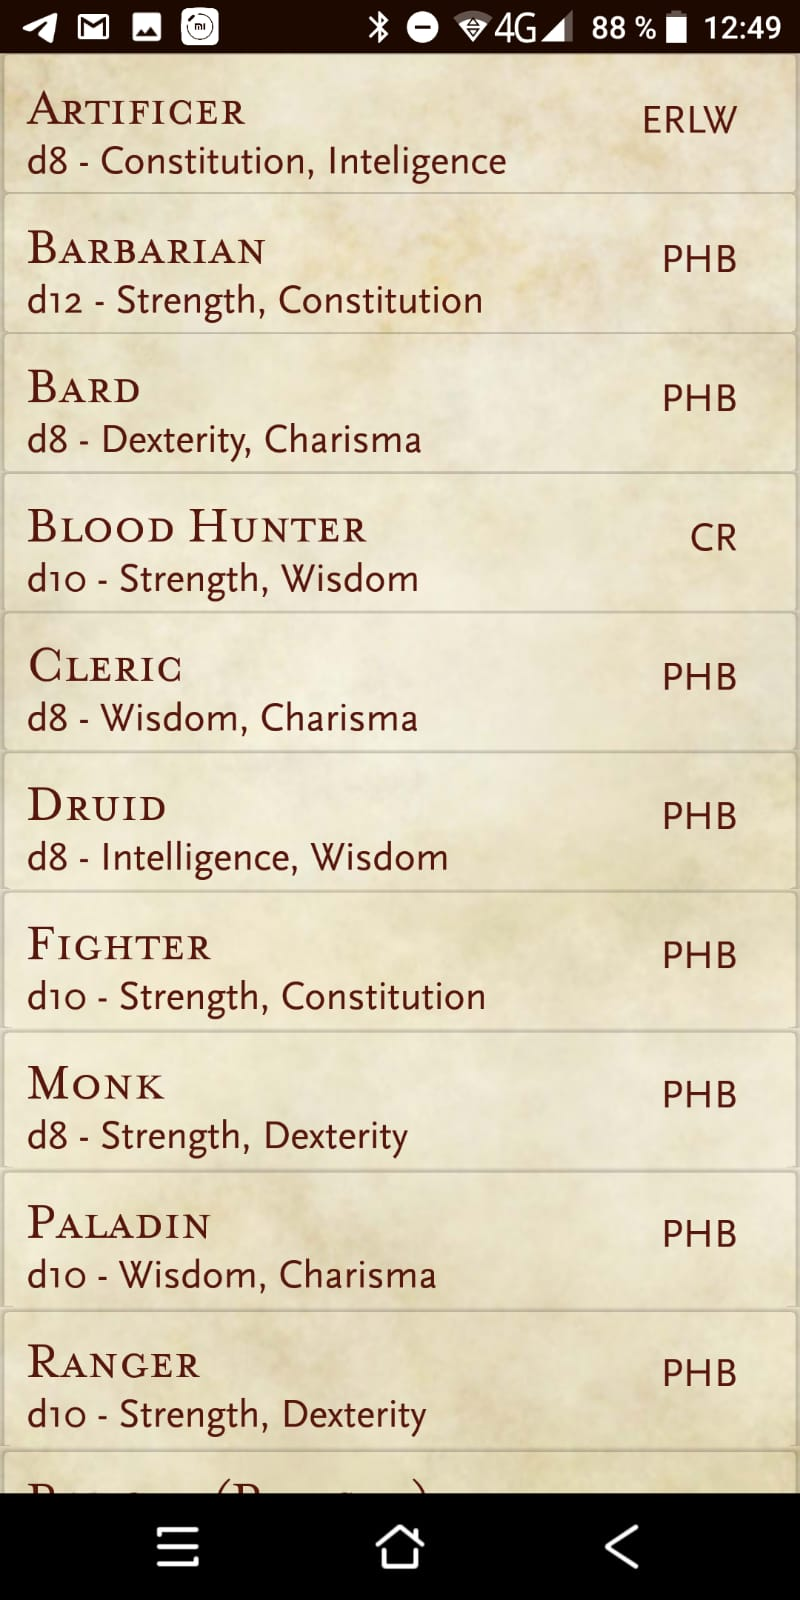
\includegraphics[width=0.5\textwidth]{Images/5e_Character_1.jpeg}
        \caption{\textit{\textbf{5e Character}}: Pantalla de selección 
        de clases}
        \label{5e_Character1}        
    \end{minipage} \hspace{2cm}
    \begin{minipage}{0.38\textwidth}
        \centering
        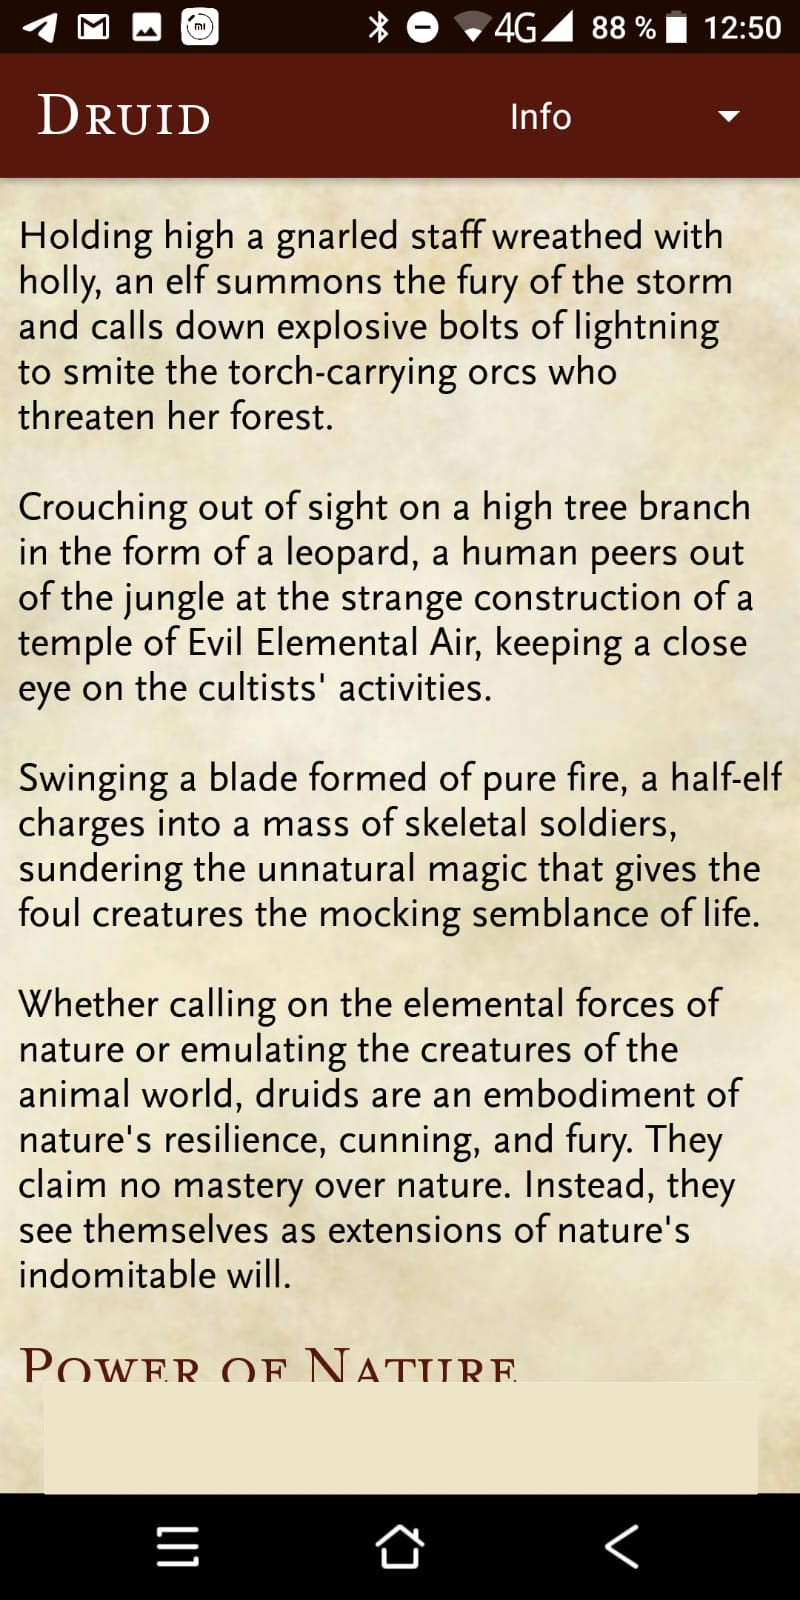
\includegraphics[width=0.5\textwidth]{Images/5e_Character_2.jpeg}
        \caption{\textit{\textbf{5e Character}}: Información 
        de la clase \textit{Druida}}
        \label{5e_Character2}        
    \end{minipage}
\end{figure}

Como en los juegos de rol se utilizan diferentes tipos de dados 
(de 3, 4, 6, 8, 10, 12, 20, 30 y hasta 100 lados), también podemos encontrar aplicaciones 
como \textit{\textbf{RPG Simple Dice}}, expuesta en las figuras \ref*{SimpleDice1} y \ref*{SimpleDice2} que están preparadas para simular los resultados 
de lanzar estos dados, lo cual hace que se conviertan en una herramienta útil si no 
disponemos de alguno de éstos.

\begin{figure}[H]
    \centering
    \begin{minipage}{0.35\textwidth}
        \centering
        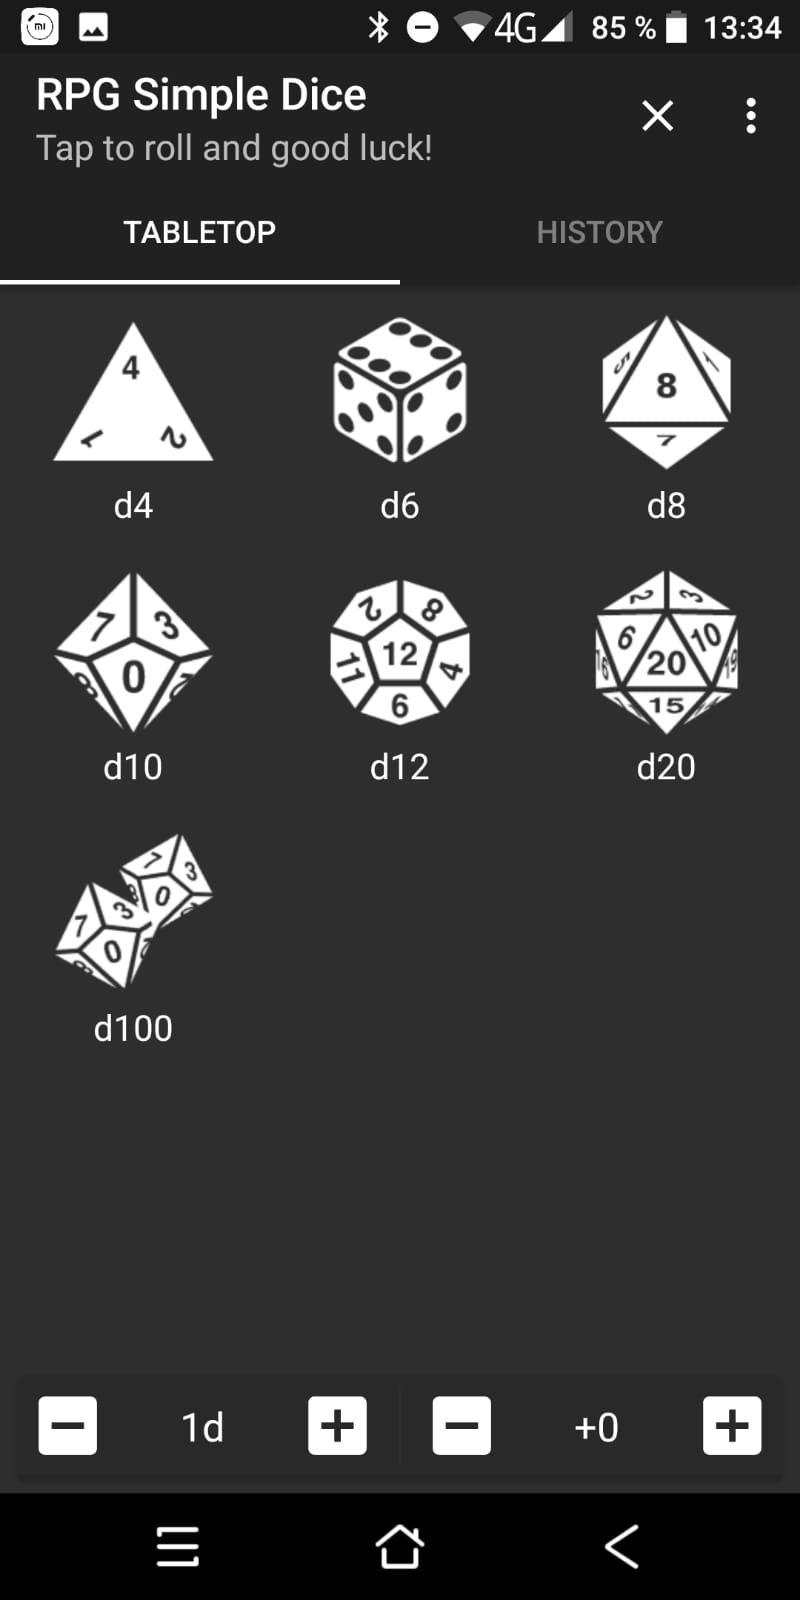
\includegraphics[width=0.5\textwidth]{Images/RPG_Simple_Dice_1.jpeg}
        \caption{\textit{\textbf{RPG Simple Dice}}: Pantalla de selección 
        de dados}
        \label{SimpleDice1}        
    \end{minipage} \hspace{2cm}
    \begin{minipage}{0.35\textwidth}
        \centering
        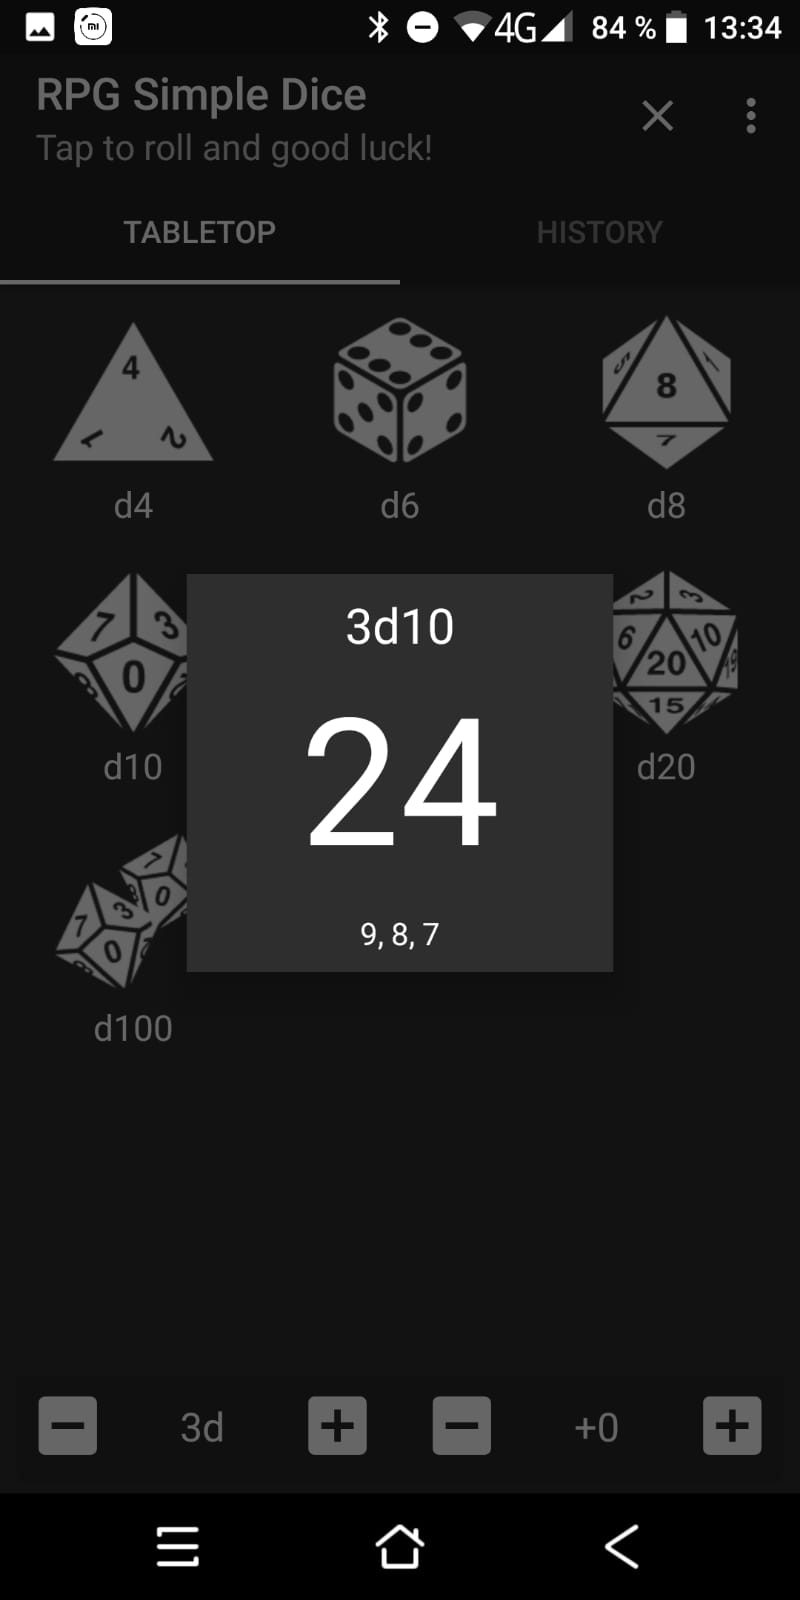
\includegraphics[width=0.5\textwidth]{Images/RPG_Simple_Dice_2.jpeg}
        \caption{\textit{\textbf{RPG Simple Dice}}: Ejemplo de lanzamiento de 
        dados}
        \label{SimpleDice2}        
    \end{minipage}
\end{figure}

Otras aplicaciones proporcionan algunas herramientas que simplifican 
cálculos que resultan tediosos durante el transcurso de la partida, como 
es el caso de \textit{\textbf{BattleTrack}}, cuya interfaz se puede apreciar 
en las figuras \ref*{BattleTrack1} y \ref*{BattleTrack2}. Dependiendo de la aplicación 
que se utilice, puede incluir su propio simulador de dados, lo que hace 
innecesario el uso de aplicaciones específicas para ello. \medskip

El punto negativo de estas aplicaciones es que son generales y no disponen de 
la información específica de los personajes de los jugadores, de manera que 
el resultado es aproximado, o requiere que el usuario especifique previamente 
toda la información, lo que puede llegar a resultar tedioso si en una partida 
se realizan múltiples cálculos de éste tipo. 


\begin{figure}[H]
    \centering
    \begin{minipage}{0.3\textwidth}
        \centering
        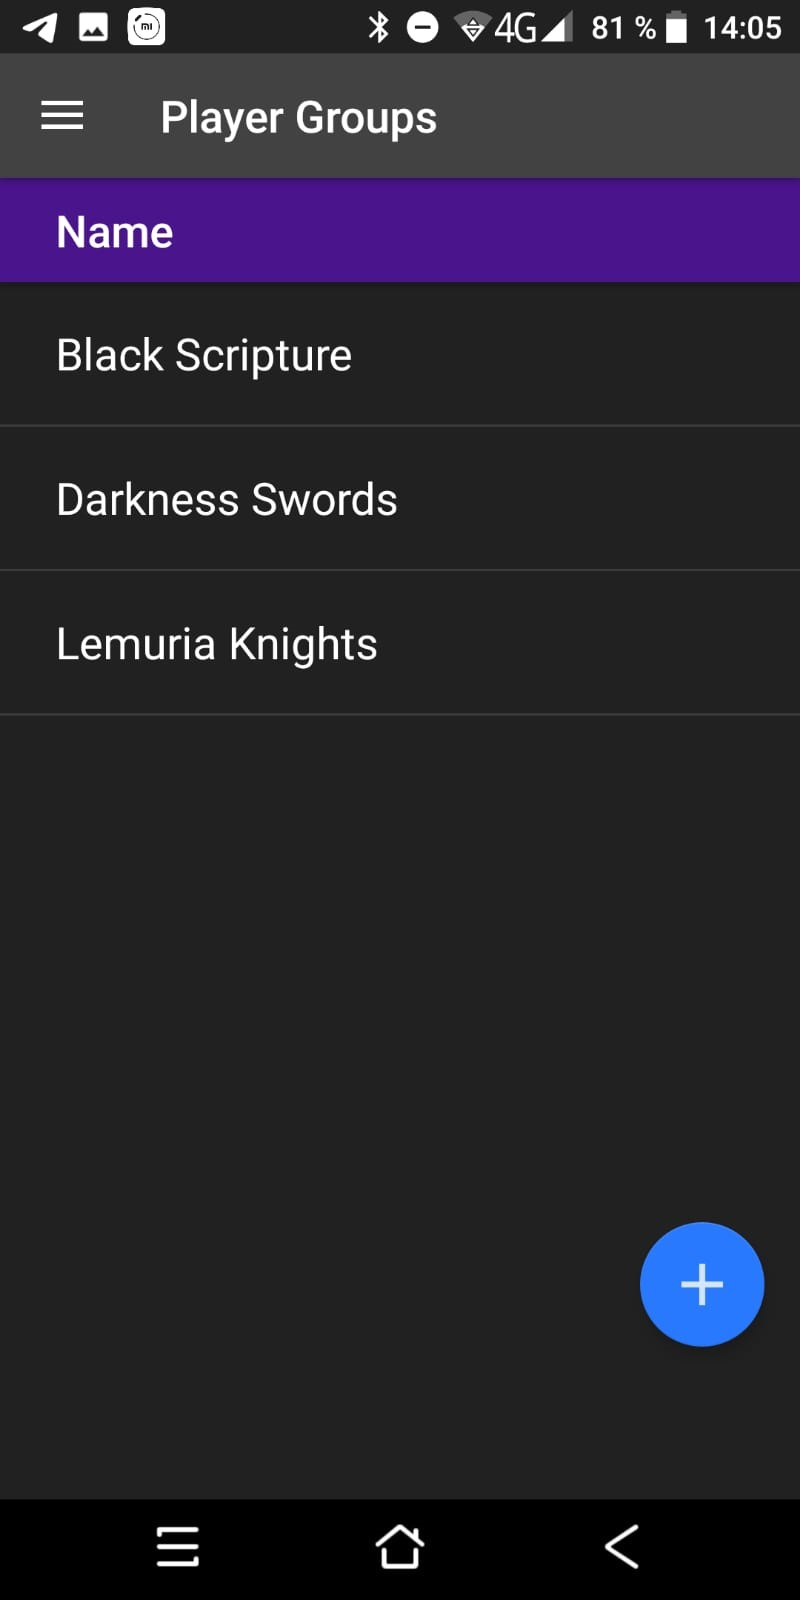
\includegraphics[width=0.7\textwidth]{Images/BattleTrack_1.jpeg}
        \caption{\textit{\textbf{BattleTrack}}: Pantalla de grupos }
        \label{BattleTrack1}   
        
    \end{minipage} \hspace{2cm}
    \begin{minipage}{0.3\textwidth}
        \centering
        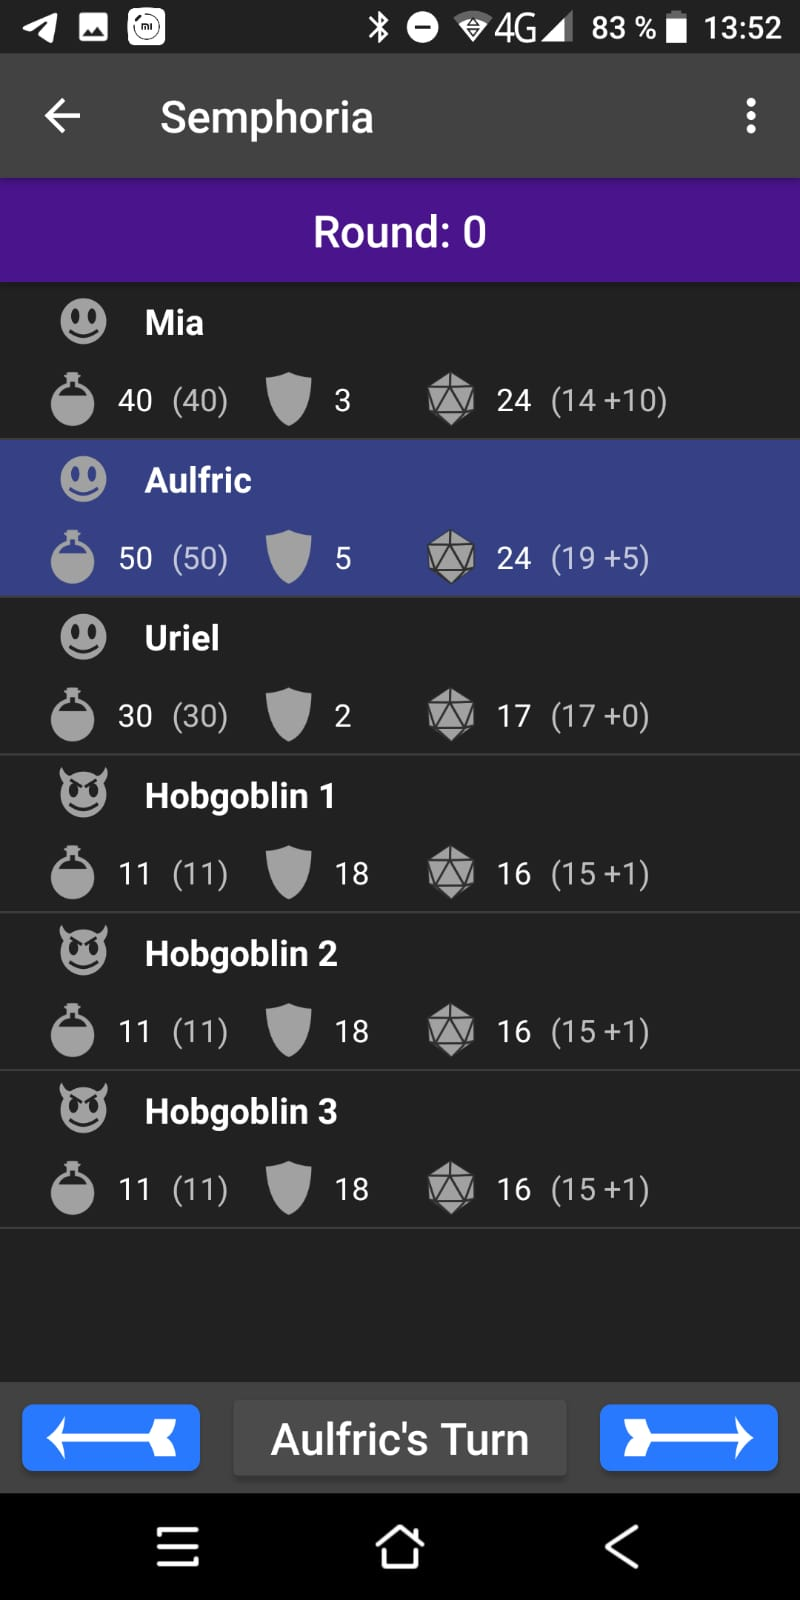
\includegraphics[width=0.7\textwidth]{Images/BattleTrack_2.jpeg}
        \caption{\textit{\textbf{BattleTrack}}: Ejemplo de combate}
        \label{BattleTrack2}           
    \end{minipage}
\end{figure}

Con el fin de ayudar en la ambientación, aplicaciones como 
\textit{\textbf{RPGSound}} (Figuras \ref*{RPGSound1} y \ref*{RPGSound2}) 
aportan bibliotecas de sonido que se pueden 
utilizar durante la representación de la partida para sumirse en ella.
 
\begin{figure}[H]
    \centering
    \begin{minipage}{0.3\textwidth}
        \centering
        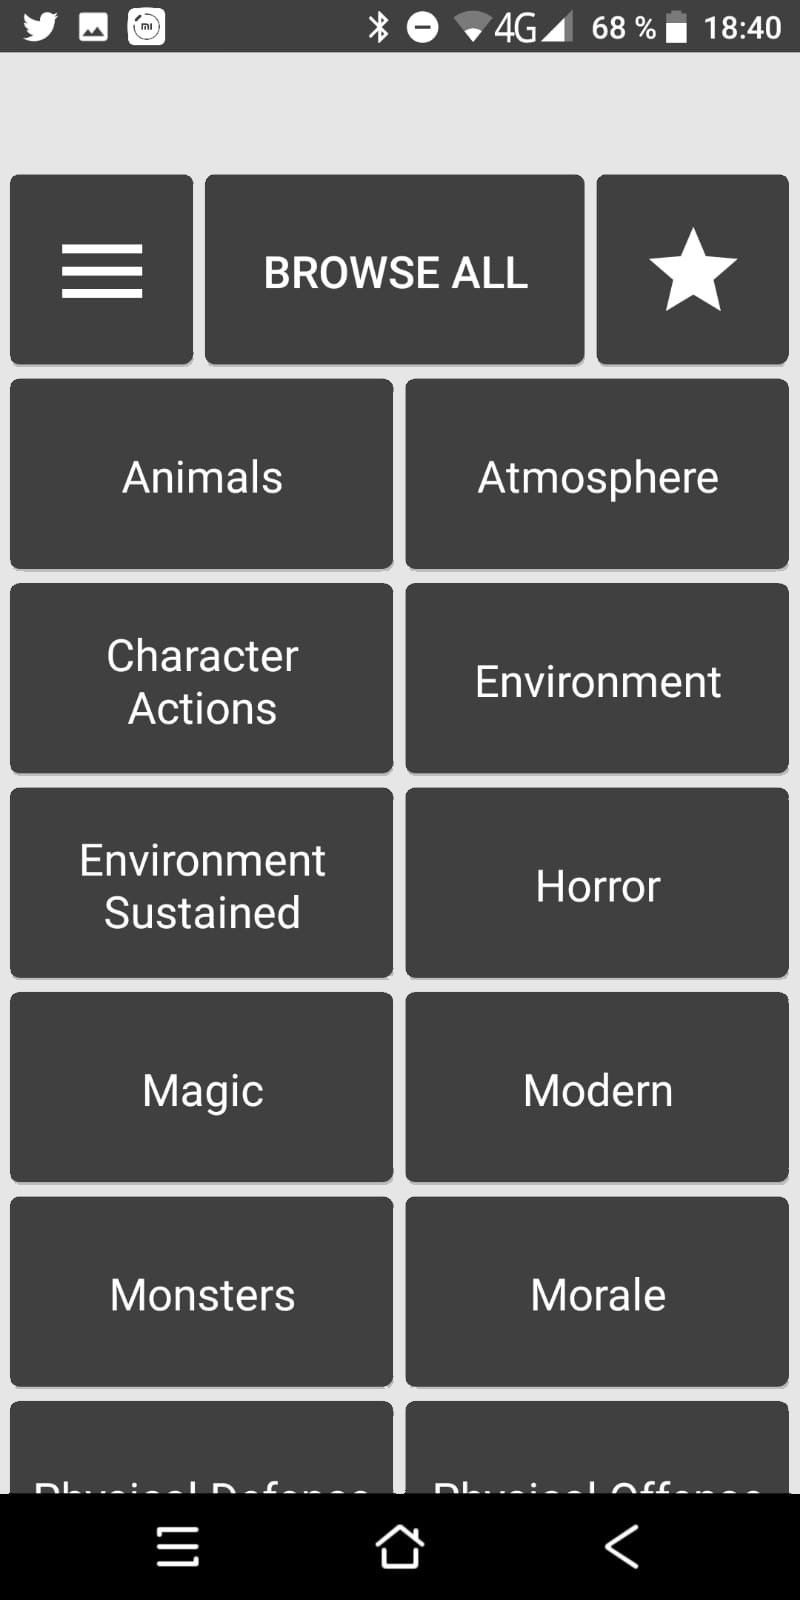
\includegraphics[width=0.7\textwidth]{Images/RPGSound_1.jpeg}
        \caption{\textit{\textbf{RPGSound}}: Menú principal}
        \label{RPGSound1} 
    \end{minipage} \hspace{2cm}
    \begin{minipage}{0.3\textwidth}
        \centering
        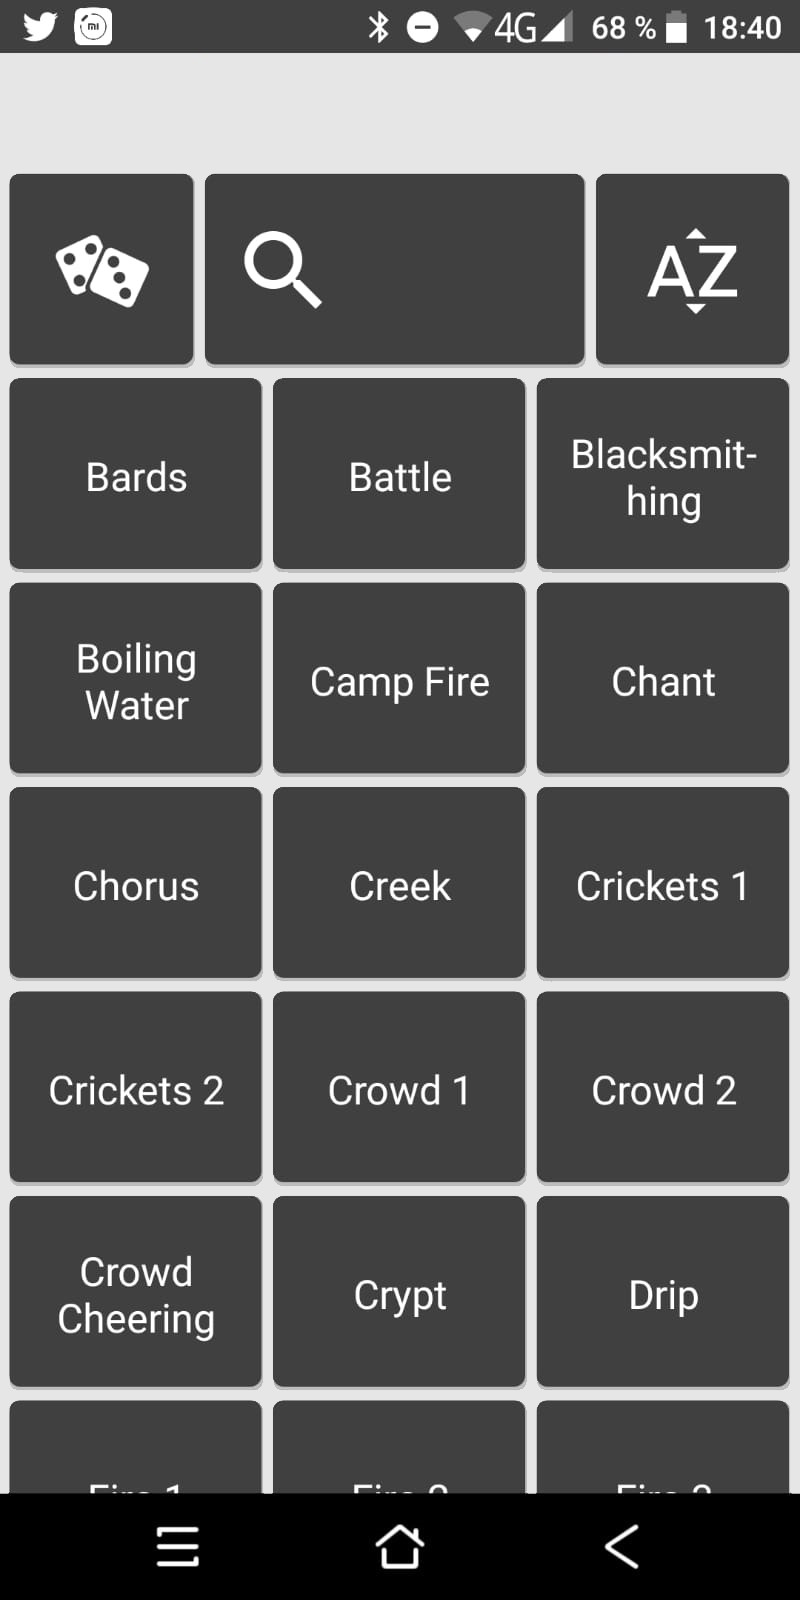
\includegraphics[width=0.7\textwidth]{Images/RPGSound_2.jpeg}
        \caption{\textit{\textbf{RPGSound}}: Menú de \textit{Ambiente}}
        \label{RPGSound2} 
    \end{minipage}
\end{figure}

Finalmente, quedan las aplicaciones conocidas como \textit{generadores de
personaje}, que permiten al usuario crear personajes para formar parte de 
una partida de rol, y acceder a esa información de forma rápida. Un buen 
ejemplo de esto es \textit{\textbf{RPG Character Sheet}}, como se muestra en 
las figuras \ref*{RPGCharacterSheet1} y \ref*{RPGCharacterSheet2}. Aunque estas aplicaciones 
suelen reunir las funcionalidades de la mayoría de las aplicaciones previamente 
explicadas, suelen tener una interfaz bastante caótica, lo que resulta en una 
curva de aprendizaje bastante elevada para usuarios nuevos, que acaban 
prefiriendo el método tradicional, o el uso de varias aplicaciones más sencillas.

\begin{figure}[H]
    \centering
    \begin{minipage}{0.3\textwidth}
        \centering
        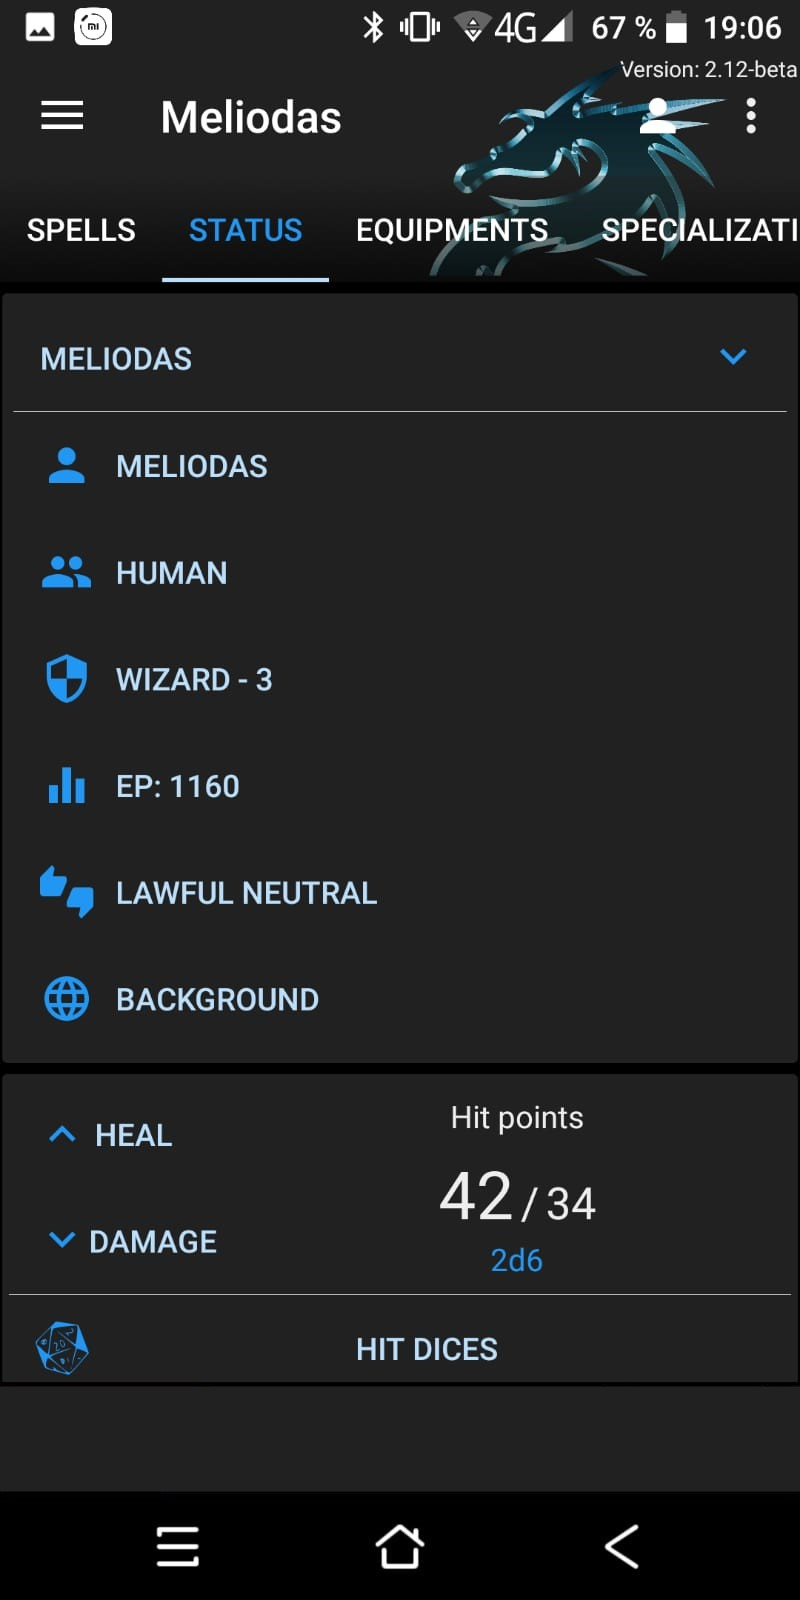
\includegraphics[width=0.7\textwidth]{Images/RPG_Character_Sheet_1.jpeg}
        \caption{\textit{\textbf{RPG Character Sheet}}: Pantalla de \textit{Estado}}
        \label{RPGCharacterSheet1}
    \end{minipage} \hspace{2cm}
    \begin{minipage}{0.3\textwidth}
        \centering
        
\includegraphics[width=0.7\textwidth]{Images/RPG_Character_Sheet_2.jpeg}
        \caption{\textit{\textbf{RPG Character Sheet}}: Pantalla de \textit{Features}}
        \label{RPGCharacterSheet2}
    \end{minipage}
\end{figure}

En resumen, hay un amplio abanico de aplicaciones que buscan resultar de utilidad a los 
jugadores de \textit{RPG} de diferentes maneras, ya sea facilitando la búsqueda de información, 
realizando los cálculos de los valores finales de las tiradas de dados o generando la información
de los personajes que forman parte de la partida.

% Import Section%
% ARPEGOS:  Automatized Roleplaying-game Profile Extensible Generator Ontology based System %
% Author : Alejandro Muñoz Del Álamo %
% Copyright 2019 %

% Section 2.2: Crítica al estado del arte %

\section{Crítica al estado del arte}
Tal y como se ha comentado previamente, existe un holgado abanico de 
aplicaciones cuya meta es mejorar y/o simplificar aspectos en lo referente a 
los juegos de rol, y aunque cumplen con su propósito, a veces no resultan 
tan efectivas como debieran. 
\medskip 

Esto puede deberse a que tras dedicar el tiempo y esfuerzo necesarios para 
desarrollar la aplicación, el estudio del juego ha aprovechado ese tiempo 
de producción para revisar el juego y editarlo, realizando modificaciones 
que provocan que \emph{\textbf{la aplicación quede obsoleta en poco tiempo}}. 
\medskip

Otro inconveniente es que las aplicaciones que requieren mucha información 
específica, como los generadores de personaje, pueden llegar a 
\emph{\textbf{resultar muy complejas}}, y al tener una interfaz poco intuitiva, 
provoca que el usuario no experimentado considere que el esfuerzo que tiene que 
dedicar para aprender cómo utilizarla es mayor que el de realizar el proceso manualmente. \medskip

También existen aplicaciones que no contemplan la reutilización de la 
información que han producido para efectuar operaciones que mejoren 
la jugabilidad, por lo que el usuario no le ve provecho a emplear dichas
aplicaciones.

% Import Section %
% ARPEGOS:  Automatized Roleplaying-game Profile Extensible Generator Ontology based System %
% Author : Alejandro Muñoz Del Álamo %
% Copyright 2019 %

% Section 2.3: Propuesta %

\section{Propuesta} \label{Propuesta}
Tras analizar el estado del arte, y destacar algunos de los aspectos negativos de éste, lo que prosigue es diseñar una 
propuesta que permita recoger las mejores ideas de las herramientas actuales, y que además pueda dar solución a los 
problemas comentados en el apartado \ref{Critica_Estado_Arte} (\textit{Crítica al estado del arte}). \medskip

\subsection{Plataforma} \label{Plataforma}
En primer lugar, se debe considerar cuál será la plataforma en la que se implementará la aplicación, puesto que es la base 
sobre la que se realiza el desarrollo, y que condiciona las herramientas que se pueden utilizar para la elaboración del proyecto. 
\medskip

Como se puede apreciar en la sección \ref{Estado_Arte} (\textit{Estado del arte}), muchas de las aplicaciones existentes 
se desarrollan en entornos móviles, lo que supone que la aplicación pueda ser accesible desde cualquier sitio. Por otro lado, 
se considera una opción plausible el poder extender la aplicación a otros entornos, tales como sistemas de sobremesa, o el entorno 
web. Teniendo todo esto en consideración, se ha tomado la decisión de realizar una \textbf{aplicación móvil}, haciendo uso de 
\textbf{herramientas de desarrollo multiplataforma}, de manera que en un futuro sea posible extender el proyecto a otras plataformas.

\subsection{Arquitectura} \label{Arquitectura}
Después de seleccionar la plataforma principal de desarrollo, el siguiente paso es definir la arquitectura de la aplicación, 
que hace referencia a \textit{“la estructura general de este y a las formas en las que ésta da integridad conceptual a un 
sistema.”} \autocite*{Shaw1995}. Como explica Cardacci \autocite*{Addati2013}, con el tiempo se han ideado una amplia 
variedad de formas arquitectónicas, con el objetivo de separar los diferentes desafíos que plantea el desarrollo de software 
conceptualmente, y lograr cierto grado de independencia entre los elementos que componen el software, de manera que los cambios 
realizados en uno no tenga efecto en el resto. \medskip

De entre todas las posibilidades existentes, hemos optado por utilizar el patrón \textit{Modelo-Vista-Modelo de Vista} (\textbf{MVVM})
\autocite*{MicrosoftMVVM}, que separa el software en tres componentes: \textit{modelo}, \textit{modelo de vista} y \textit{vista}.\medskip

\begin{figure}[H]
    \centering
    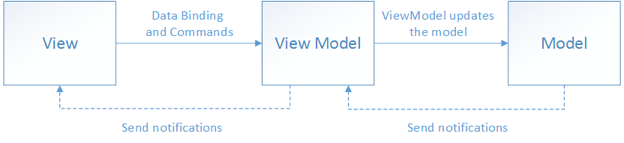
\includegraphics[width=10cm]{Images/mvvm.png}
    \caption{Patrón MVVM: \textit{Modelo-Vista-Modelo de Vista}. \smallskip Extraído de \textit{Microsoft Docs} \autocite*{MicrosoftMVVM}}
\end{figure}

\subsection{Modelo de datos} \label{Modelo_Datos}
Como definen Pérez y Gardey \autocite*{Perez2017}, un modelo de datos es un esqueleto estructural que permite organizar 
y documentar la información. Esta estructura busca definir el acceso y el almacenamiento de los datos de forma 
unívoca, de manera que permitan la comunicación entre las aplicaciones que hagan uso de los datos del modelo. \medskip

\begin{figure}[H]
    \centering
    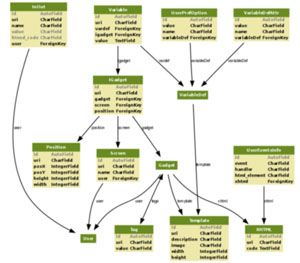
\includegraphics[width=5cm]{Figures/modelo_datos.jpg}
    \caption{Esquema de un modelo de datos. Extraído de \textit{definición.de} \autocite*{Perez2017}}
\end{figure}

Para este proyecto hace falta un modelo de datos que permita representar diversos mundos, y establecer relación entre sus elementos.
Por ello, se ha tomado la decisión de plantear un modelo \textbf{ontológico}. Citando a Muñoz y Aguilar \autocite*{Munoz2009}, 
\textit{“una ontología es una base de datos que describe los conceptos del mundo en un dominio específico, algunas de sus 
propiedades y cómo estos conceptos se relacionan entre sí”}. \autocite*{Munoz2009}
 


% Import Section %
% ARPEGOS:  Automatized Roleplaying-game Profile Extensible Generator Ontology based System %
% Author : Alejandro Muñoz Del Álamo %
% Copyright 2019 %

% Section 2.4: Metodología %

\section{Metodología} \label{Metodologia_Desarrollo}
\subsection{Metodologías de desarrollo software}
El desarrollo de software está en constante cambio. Esto se debe en parte a la continua aparición de nuevas tecnologías que 
transforman los modelos teóricos vigentes. Por otro lado, existe una barrera entre las herramientas de desarrollo y la 
metodología que impide la puesta en práctica de muchos de los modelos propuestos. No es fácil adaptarse de manera adecuada 
a una metodología de desarrollo de software, lo que resulta en un proceso con posibles demoras. No obstante, 
\textit{el uso de una metodología adecuada ha probado ser un pilar para el desarrolllo de un proyecto de construcción de software} \autocite*{Moyo} \medskip

De aquí es posible extraer dos ideas claras: la primera es que adaptarse a una metodología es una tarea complicada, 
pero que de lograrse con éxito, son claros los beneficios obtenidos frente a los resultados si no se hubiera 
realizado dicha adaptación. La segunda es que resulta necesario realizar un estudio para conocer 
cuáles son las métodologías existentes, cuáles están presentes en el mercado, conocer sus ventajas e inconvenientes, 
conocer su proceso de implementación y conocer si su alcance está alineado con el objetivo que se desea lograr. \medskip

Actualmente existe un gran abanico de metodologías, las cuales se adaptan en mayor o menor medida al tipo de producto 
que se pretende desarrollar. La gran mayoría de ellas están basadas en alguno de los siguientes modelos de desarrollo 
de software:
\begin{itemize}

    \item \textbf{Desarrollo en cascada}: Pressman \autocite*{Pressman1988} plantea el desarrollo en cascada como el 
    método que ordena las etapas de desarrollo de forma directa, de manera que cada etapa se inicia tras la finalización 
    de la anterior.
    
    Como expresa Prieto \autocite*{PrietoAlvarez2013}, aplicar esta metodología muestra beneficios cuando cada fase de desarrollo 
    dispone del tiempo necesario para llevarse a cabo. Prieto también comenta que para reducir los riesgos, es necesario tener 
    establecidos los requisitos del proyecto claramente desde el principio del proyecto.

    \begin{figure}[H]
        \centering
        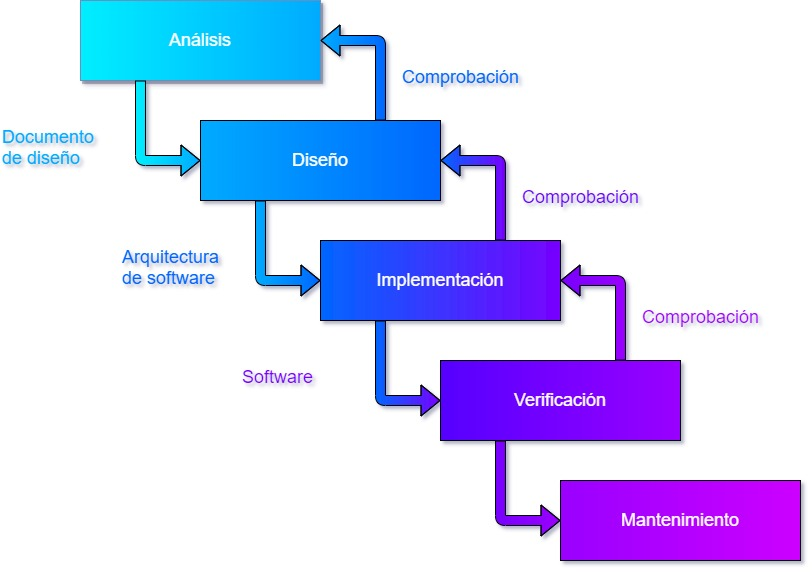
\includegraphics[width=5cm]{Figures/modelo_cascada.jpg}
        \caption{Modelo de desarrollo en cascada. Extraido de \textit{(IONOS)}\autocite*{DigitalGuideIONOS2019}}
    \end{figure}

    \item \textbf{Desarrollo en espiral}: Este modelo permite un análisis más profundo de las etapas del desarrollo del 
    producto, de acuerdo con Prieto \autocite*{PrietoAlvarez2013}. Las actividades del modelo están dispuestas en espiral, en la que cada iteración o vuelta representa 
    un conjunto de actividades acorde a una etapa del desarrollo. El orden de las actividades queda determinado por el 
    análisis del riesgo, comenzando por el bucle interior, \medskip 


    \begin{figure}[H]
        \centering
        
\includegraphics[width=5cm]{Figures/SVG/espiral.png}
        \caption{Modelo de desarrollo en espiral. Extraído de \textit{freepng.es} \autocite*{Espiral}}
    \end{figure}

    \item \textbf{Desarrollo con prototipos}: Desde el punto de vista de Roque y col. \autocite*{RoqueHernandez2015}, el desarrollo con 
    prototipos mejora la comunicación entre el equipo de desarrollo y el cliente. Esto permite que se puedan introducir cambios con 
    facilidad y disminuya el tiempo de desarrollo. Consiste en un proceso iterativo que tiene cinco fases:

    % RAMÓN VENTURA ROQUE HERNÁNDEZ, JUAN MANUEL SALINAS ESCANDÓN, CALEB ALFREDO ÁLAMOS ACOSTA, ROBERTO ARREOLA RIVERA
    %Comparación empírica entre el proceso unificado y el desarrollo de software por prototipos. 
    \begin{enumerate}
        \item \textbf{\textit{Comunicación}}: Se indica un conjunto de objetivos que el software debe cumplir.
        \item \textbf{\textit{Plan rápido}}: Se propone una estrategia para llevar a cabo el desarrollo
        \item \textbf{\textit{Diseño rápido}}: Se realiza el diseño de una interfaz gráfica rápidamente.
        \item \textbf{\textit{Construcción}}: Se construye el prototipo del sistema software.
        \item \textbf{\textit{Entrega y retroalimentación}}: Se entrega el prototipo y el cliente realiza una 
        retroalimentación al equipo, que da inicio a una nueva iteración que incorpora los ajustes indicados en la 
        información dada por el cliente.
    \end{enumerate}\medskip
    
    \begin{figure}[H]
        \centering
        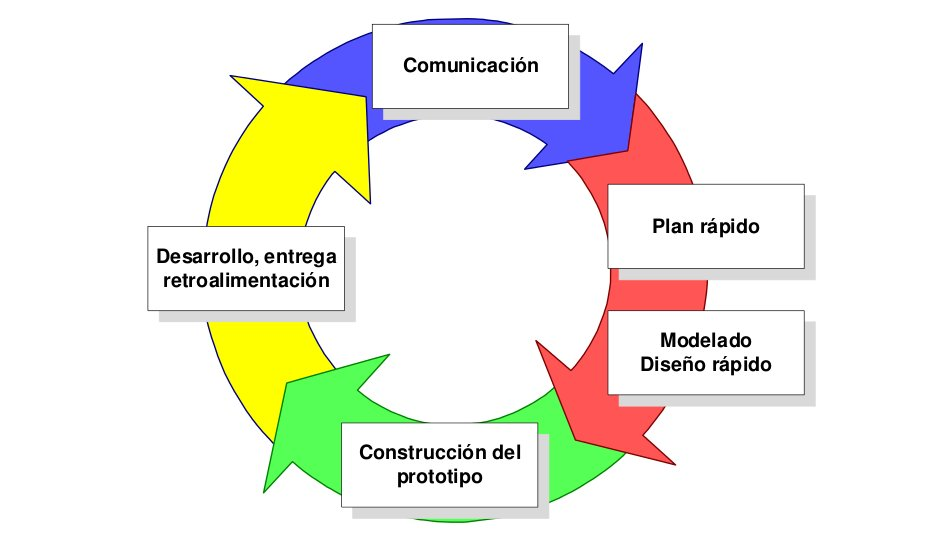
\includegraphics[width=5cm]{Figures/modelo_prototipos.jpeg}
        \caption{Modelo de desarrollo con prototipos. Extraído de \textit{sites.google.com} \autocite*{Prototipos}}
    \end{figure}

    \item \textbf{Desarrollo incremental}: Zumba \autocite*{Zumba2018} postula que el desarrollo incremental 
    está basado en la introducción por etapas (o iteraciones) de funcionalidades de la aplicación. La primera 
    iteración suele ser básica, con los elementos mínimos requeridos, y cada iteración posterior es una versión 
    entregable del proyecto, que introduce alguna funcionalidad nueva. \medskip

    \begin{figure}[H]
        \centering
        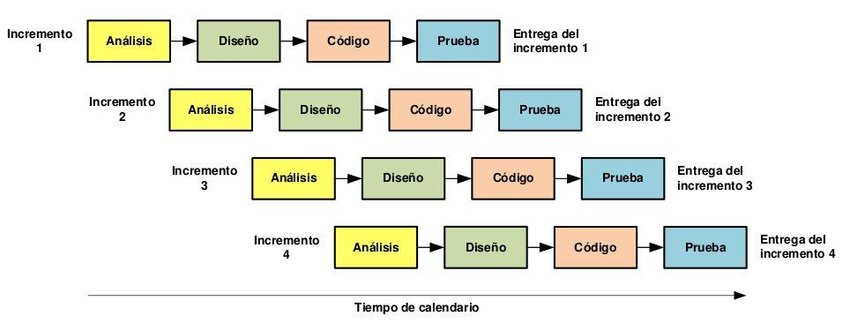
\includegraphics[width=8cm]{Figures/modelo_incremental.png}
        \caption{Modelo de desarrollo incremental. Extraído de \textit{researchgate.net} \autocite*{Alarcon2016}}
    \end{figure}
\end{itemize}

\subsection{Metodologías Ágiles}
\textit{“En febrero de 2001 nace el término \textbf{ágil} aplicado al desarrollo de software, tras una reunión celebrada en 
\textnormal{Utah (EEUU)}. El objetivo de la misma fue esbozar valores y principios que deberían permitir desarrollar 
software de manera rápida, dando respuesta a los cambios surgidos durante el desarrollo del proyecto. Se pretende 
con esto ofrecer alternativas a los procesos de desarrollo software tradicionales, rígidos y dirigidos por la documentación 
que se generaba en cada una de las etapas del proceso.”} \autocite*{AmayaBalaguera2015} \medskip

El punto de partida para ello fue el \textbf{Manifiesto Ágil} \autocite*{Beck2001}: 
documento que resume la filosofía ágil, en el cual se valoran los siguientes elementos:
\begin{itemize}
    \item \textbf{El individuo y las interacciones del equipo de desarrollo sobre el proceso y las herramientas}:
    Las personas que forman parte del proyecto son el principal factor de éxito de un proyecto, de manera que el entorno
    influye menos que la bondad del equipo que realiza el desarrollo. Es preferible que el entorno se adapte al equipo.

    \item \textbf{Desarrollo de software útil es mejor que conseguir una buena documentación}:
    La regla a seguir es \textit{producir sólo documentos que sean necesarios inmediatamente para tomar una 
    decisión importante}.

    \item \textbf{La colaboración del cliente sobre la negociación de un contrato}: Se propone una interacción 
    constante entre cliente y desarrolladores, de manera que esta colaboración permita marcar el ritmo del 
    proyecto y asegure el éxito del mismo.

    \item \textbf{Respuesta rápida a los cambios es mejor que seguir un plan de forma estricta}:
    La habilidad de responder a los cambios determina el éxito o fracaso del proyecto, de manera que lo
    más importante de la planificación es su flexibilidad.
\end{itemize} 

Los principios del \textit{Manifiesto Ágil} se basan en estos valores, que a su vez hacen de fundamentos de 
todas las metodologías ágiles, orientando el desarrollo a la rápida obtención de un producto funcional 
aunque no tenga todas sus funciones implementadas. \medskip

Del modelo de desarrollo ágil se pueden encontrar diversas metodologías, como \textbf{eXtreme Programming} \autocite*{Stephens2003},
\textbf{Scrum} \autocite*{Schwaber2011} o \textbf{Crystal Clear} \autocite*{Cockburn2004}. 
Para este proyecto se ha tomado la decisión de seguir la metodología \textit{\textbf{Scrum}} ya que debido a la naturaleza y complejidad del mismo, 
es posible que sea necesario realizar cambios en el planteamiento del proyecto durante el proceso de desarrollo. \medskip

\subsection{SCRUM}
\subsubsection{Introducción}
Empleando las palabras de Rodríguez, \textit{“\textbf{SCRUM} es una de las metodologías de desarrollo ágil más reconocidas a nivel mundial, su concepción resulta de unos 
análisis realizados por \textbf{Ikujiro} \textbf{Nonaka} e \textbf{Hirotaka} \textbf{Takeuchi} en los años 80, resaltando el trabajo en equipo para el 
desarrollo de productos y la autonomía que estos deben tener (Takeuchi \& Nonaka, 1986). Su diseño se debe a que 
en los años 90, \textbf{Jeff} \textbf{Sutherland} y \textbf{Ken} \textbf{Schwaber} formalizaron un marco de trabajo y unas reglas aplicadas 
particularmente al desarrollo de software de productos complejos.”} \autocite*{Rodriguez} \medskip 

\begin{figure}[H]
    \centering
    
\includegraphics[width=5cm]{Images/Logo_Scrum.jpeg}
    \caption{Logo de \textit{Scrum}. Extraído de \textit{worldvectorlogo.com} \autocite*{ScrumLogo}}
\end{figure}

\subsubsection{Características}
A continuación se muestra una serie de características que deben tener todos los procesos que se introducen al marco 
de la metodología \textit{Scrum}:
\begin{itemize}
    \item El desarrollo incremental de los requisitos en bloques temporales cortos y fijos.
    \item Se da prioridad los requisitos más valorados por el cliente.
    \item El equipo se sincroniza diariamente y se realizan las adaptaciones necesarias.
    \item Tras cada iteración se muestra el resultado real al cliente, para que tome las decisiones 
    necesarias en relación al resultado observado.
    \item Se le da al equipo la autoridad necesaria para poder cumplir los requisitos.
    \item Fijar tiempos máximos para lograr objetivos.
    \item Equipos de trabajo pequeños (de 5 a 9 personas).
\end{itemize}

\subsubsection{Ciclo de desarrollo}
Para entender el ciclo de desarrollo de \textit{Scrum} es necesario conocer las fases que lo definen:
\begin{enumerate}
    
    \item \textbf{Planificación}: Reunión de los involucrados en la que se definen los requisitos prioritarios para 
    la iteración actual y se elabora una lista de tareas necesarias para lograr los requisitos previamente seleccionados.

    \item \textbf{Scrum diario}: Evento del equipo de desarrollo de quince minutos, que se realiza diariamente durante la
    ejecución de la iteración para explicar lo que se ha alcanzado desde la última reunión, lo que se hará antes de la 
    siguiente y los obstáculos que se han presentado. 

    \item \textbf{Revisión}: El equipo presenta al cliente los requisitos completados en la iteración. En función de los 
    resultados mostrados y de los cambios habidos en el contexto del proyecto, el cliente realiza las adaptaciones 
    necesarias de manera objetiva, replanificando el proyecto.

    \item \textbf{Retrospectiva}: El equipo analiza cómo ha sido su manera de trabajar y qué problemas podrían impedirle 
    progresar adecuadamente, mejorando de manera continua su productividad.
\end{enumerate}

\begin{figure}[H]
    \centering
    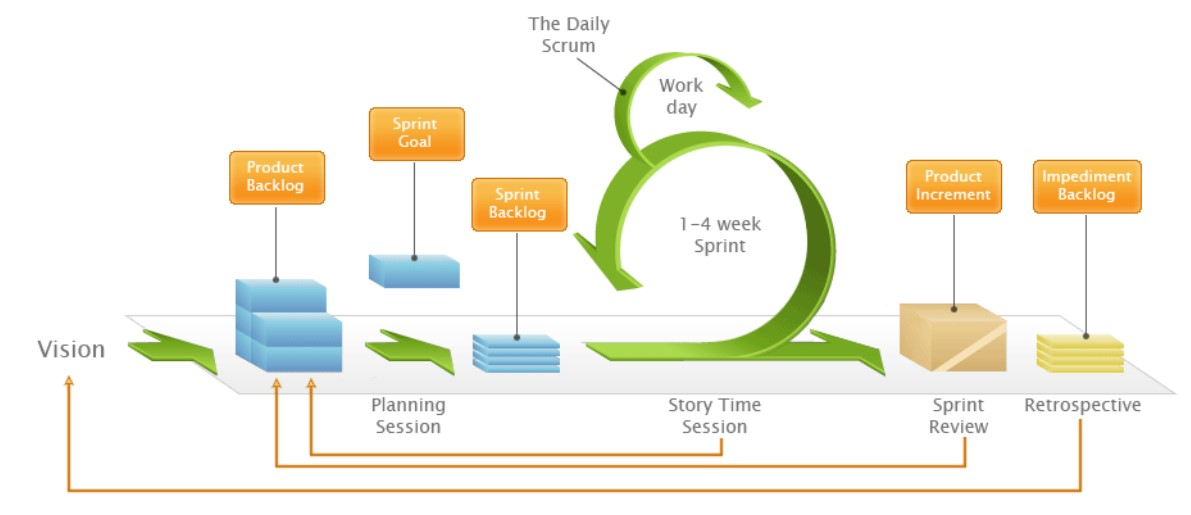
\includegraphics[width=14cm]{Images/Ciclo_Scrum.jpg}
    \caption{Ciclo de desarrollo de \textit{Scrum}. Extraído de \textit{Metodología Scrum} \autocite*{TrigasGallego2012}}
\end{figure}

\subsubsection{Roles}
Los roles presentes en \textit{Scrum} son los siguientes:
\begin{itemize}
    \item \textbf{Product Owner}: Tiene la responsabilidad de decidir qué trabajo necesita hacerse, y maximizar el valor 
    del proyecto o producto que se esté llevando a cabo. Para ello debe tener las siguientes cualidades:
    \begin{enumerate}
        \item \textit{Saber gestionar prioridades}: Es responsable de gestionar los presupuestos, de contratar al equipo de 
        desarrollo y de explicar cuál es el valor que produce el producto en el que está invirtiendo.
        \item \textit{Toma de decisiones}: Debe ser capaz de tomar decisiones por su cuenta.
        \item \textit{Coordinador}: Tiene que poder medir el valor generado y utilizar la flexibilidad de entregar cada 
        \textit{sprint} para incrementar ese valor.
    \end{enumerate}
    
    \item \textbf{Scrum Master}: Persona que ayuda al equipo y a la organización a optimizar el uso de la 
    metodología. Traslada la visión del proyecto al equipo, y elimina los obstáculos que impiden que el equipo alcance el 
    objetivo del \textit{sprint}.

    \item \textbf{Development Team}: Grupo de profesionales con los conocimientos técnicos necesarios y que desarrollan el proyecto de manera
    conjunta llevando a cabo los requisitos a los que se comprometen al inicio de cada \textit{sprint}.
\end{itemize}

\begin{figure}[H]
    \centering
    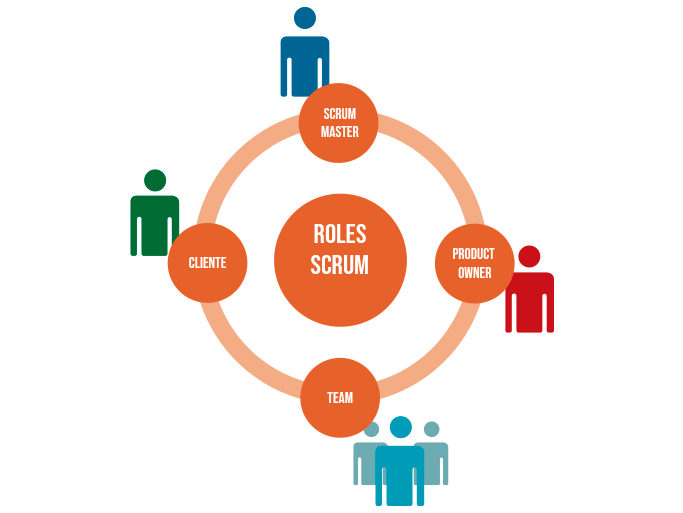
\includegraphics[width=10cm]{Images/roles.png}
    \caption{Roles en \textit{Scrum}. Extraido de \textit{herizont.com} \autocite*{ScrumRoles}}
\end{figure}

% Import Section %
% ARPEGOS:  Automatized Roleplaying-game Profile Extensible Generator Ontology based System %
% Author : Alejandro Muñoz Del Álamo %
% Copyright 2019 %

% Section 2.4: Resumen %
\section{Resumen}
Las aplicaciones actuales permiten generar información útil para los jugadores de rol, tal como referencias rápidas, 
tiradas de dados, resultados de combates e incluso la información de sus personajes. Pero la mayoría de ellas están limitadas
en que su ámbito suele estar reducido a una única versión de un juego específico. Además, no pueden personalizarse para el jugador, 
o requieren que se introduzca la información a mano cada vez que se utilizan, resultando ser menos práctico que el método tradicional.
\medskip

En relación a esto, es de gran interés promover el uso de ontologías en este tipo de aplicaciones, como este proyecto, por ejemplo, 
pues permiten relacionar elementos de diferentes ontologías entre sí, permitiendo reutilizar elementos ya definidos, y ampliar
modelos de datos sin realizar modificaciones de las versiones previas, posibilitando el uso de nuevas versiones de los modelos
sin alterar los ya existentes, facilitando al usuario la posibilidad de escoger la versión que considere más adecuada para cada ocasión.
\medskip

Por otro lado, con respecto al desarrollo de este proyecto se ha decidido optar por la metodología \textit{Scrum} porque 
permite al equipo de desarrollo trabajar con requisitos concretos a corto plazo, priorizando los requisitos más valorados 
por los clientes, y que permite a éstos últimos disponer de resultados al final de cada iteración, de manera que pueden 
tomar las decisiones que consideren oportunas para la siguiente iteración del desarrollo.


